\documentclass{beamer}
%\usetheme[
%          titlepagelogo=bold50-illinois,% Logo for the first page
%          pageofpages=of,% String used between the current page and the total page count
%          titleline=true,% Show a line below the frame title
%          ]{TorinoTh}

\usetheme{Luebeck}

\usepackage{beamerthemesplit}
\usepackage{graphics}
\usepackage{graphicx}
\usepackage{hyperref}
\usepackage{comment}
\usepackage{ulem}
\usepackage{color}
\usepackage{xspace}

\newcommand{\bllt}{\item \small}
\newcommand{\doneTask}[1]{\item \small \sout{#1}}

\newcommand{\MyName}{Vivek~Kale}

\newcommand{\fixme}[1]{\textcolor{blue}{[FIXME: #1]}}
\newcommand{\revision}[1]{\textcolor{blue}{[FIXME comment : #1]}}

\newcommand{\comments}[1]{}

\title{Toastmaster's Speech}
\author{\MyName}
\date{\today}

\title[Toastmaster]{Toastmaster's Speech}
\author[Vivek Kale]{%
  Vivek~Kale\inst{1}}
\institute[University of Illinois at Urbana-Champaign]{
  \inst{1}%
  Department of Computer Science\\
  University of Illinois at Urbana-Champaign
}
\date[DLT 2014]{\today}
\subject{Comm}

%\pgfdeclaremask{ILLINOIS}{bold50}
%\pgfdeclareimage[mask=ILLINOIS,width=1cm]{bold50}{bold50}
%\logo{\vbox{\vskip0.1cm\hbox{\pgfuseimage{bold50}}}}

\begin{document}

%\AtBeginSection[]
%{
%\begin{frame}
%\frametitle{Outline}
%\tableofcontents[part=1, pausesections]
%\end{frame}
%}
%\titlepage

%\section{Toastmaster's Speech}
%\begin{frame}
\frametitle{Opening}
\begin{itemize}
\item Shake hands 
\item Ladies and Gentleman, Distinguished Members and Guests 
\end{itemize}
\end{frame} 

\begin{frame}
\frametitle{Introduction}
\begin{itemize}
\item \small Tennis is one of the world's major sports, w/ 4 grand
  slam events (the largest being Wimbledon). 
\item \small Hi, my name is Vivek and  I am going to tell you about my passion for tennis. 
\item \small I believe it has played an important role in my life. 
\item \small After this talk, I hope you will get to know how exactly tennis has shaped my mind and my view of life. 
\end{itemize} 
\end{frame} 

\begin{frame} 
\frametitle{My Perspective of Tennis Basics}
\begin{itemize} 
\item \small serve
\item \small forehand  
\item \small backhand  
\item \small volley
\item \small run to get to ball
\item \small most importantly, don't smash racket at end of point. 
\item \small To play a point in a match, you need to be able to put these all together.  \\
\end{itemize}  
\end{frame} 

\begin{frame} 
\frametitle{ Styles of Play (Everyone's has different skills that they are stronger/weaker at, and one should play a style that capitalize on strengths)  }

\begin{enumerate} 
%\item \small \textbf{Roger Federer:}
%  \begin{itemize}
%    \item \tiny has a well-balanced strategic game, and likes to serve and volley. 
%    \item \tiny Can't run as hard for long periods of time, so gets a bit offset in long matches.   
%  \item \tiny
%  \end{itemize}

%\item \small \textbf{Rafael Nadal: }
%\begin{itemize}
%  \item \tiny plays a defensive game from the baseline. 
%  \item \tiny Runs very hard, which allows him to win long matches. 
%\end{itemize}
\item \small \textbf{My Style} 
\begin{itemize}
\item \tiny Earlier on, I tried to run around a lot, as I had more time to work out. I didn't play with as much strategy through, as I was inexperienced. 
\item \tiny Now, I don't run around as much and play a  bit more offensive, as I don't have as much time to work out. I  play more strategy, as I am more experienced.  
\end{itemize} 
\end{enumerate}
\end{frame} 

\begin{frame}
\frametitle{Matches played} 
\begin{enumerate}
\item \small \textbf{7 hours match:}
\begin{itemize}
\item \tiny played defensive game, with each point lasting what seemed to be a lifetime. 
\item \tiny I amazingly won, as I simply outdid my opponent in terms of skills.
\item \tiny This taught me how important it is to know the fundamentals. One mis-hit, and I would lose the point. 
\end{itemize} 

\item \small \textbf{2 hour match:}
\begin{itemize}
\item \tiny Lost match easily to someone who was much better than me. 
\item \tiny Points were short, with me failing at several points, and the other person pinning me down at my weaknesses and using smart strategies to win.  
\item \tiny Learned that it's important to keep some good strategies to really be competitive, and not simply have good skills. 
\end{itemize}
\item \small \textbf{3.5 hour match:}
\begin{itemize} 
\item \tiny I was losing badly in first set. 
\item \tiny I then changed up my strategy,  and found some weaknesses in my opponents game. 
\item \tiny I went on to win that match.  I learned that one shouldn't just play to one's strengths, but also play with the other person's weaknesses in mind. 
% staying calm and keeping a good attitude is helpful to get out of bad situations. 
\end{itemize}
\end{enumerate}
\end{frame}

\begin{frame} 
\frametitle{Tennis is a lot like life} 
\begin{itemize}  
\item \small Trying to win a tennis match is similar to accomplishing one's goals in life.
\item \small One example of a recurring goal in my life is publishing research papers.   
\item \small Just like in a tennis match: know several basic skills. 
%For publishing a CS conference, we should know about
%  experimentation and data analysis. 

\item \small As in a tennis match, there are several working styles we might have in achieving these goals, and we chose our styles based on our strengths. 
% goals, and each style is different based on the
%  individual. 
%When we write our papers, we focus more on theory if
%that is our strength, and focus more on experimentation if that is
%our strength.  
\item \small Just like in a tennis match: experience with reaching goals
builds our ability to achieve future goals. 
% We may not publish some papers, but we learn through experience how
% to publish. 

\item \small I watched a grand slam tennis match a few days ago. It got me motivated to achieve 
a new goal, which is becoming better at public speaking. I may have ups and downs, but 
I'm hoping I can achieve this goal in the next few months. 
\end{itemize} 
\end{frame}

\begin{frame}
\frametitle{Closing}
\begin{itemize}
\item Shake hands 
\item Sit back down.
\end{itemize}
\end{frame} 

\begin{frame}
\frametitle{Delivery Notes}
\begin{enumerate}
\item \small Make sure points are all logically connected.  Ensure that each point is part of bigger picture.
\item \small memorize speech intro.
\item \small memorize speech conclusion.
\item \small rehearse transitions
\item \small memorize points in speech. 
\item \small practice delivery
\begin{itemize}
\item \tiny don't be afraid to pause after each point (helps avoid restarts)
\item \tiny \textbf{shout}  
\item \tiny don't look down
\item \tiny avoid moving hands. 
\item \tiny don't pace. 
\end{itemize}
\end{enumerate}
\end{frame} 


\begin{frame}  
\frametitle{Verbal: Intro} 
Tennis is one of the \textbf{major sports of the world}, with
\textbf{4 grand slam} events each year.  \textbf{Hi my name Vivek, and
  today} I want to tell you a bit about \textbf{my interest in
  tennis}. I believe it has \textbf{been an important part of my life}.
At the end of this talk, I hope you'll get to know how tennis has \textbf{shaped my mind}
and \textbf{my view of life}. 

\end{frame}




\begin{frame}
\frametitle{Verbal: Conclusion}

Playing a tennis match  is a \textbf{lot like trying to achieve one's
  goals} in life. One example of a goal in my life is \textbf{writing
  research papers}. Just like a tennis match, it's important to know
\textbf{basic skills such as theory, experimental analysis, and
  computer programming}.  Just like in a tennis match, it's important
to \textbf{chose your research style based on your strengths}. Just
like a tennis match, it's important to \textbf{learn from results in
  past research paper submissions to get a better chance of publishing
  in upcoming conferences}.  I \textbf{watched} a grand slam tennis
match a few days ago. It got me motivated to \textbf{achieve a new
  goal} -- getting better at public speaking. I may have \textbf{ups
  and downs} like in a tennis match, but I'm hoping that \textbf{I can
  learn from my mistakes} and achieve this goal in the \textbf{next
  few months}. 


\end{frame}


% went to florida to visit family 
% He learned something that he didn't expect
% he's going to share with you what 



%General Goal: to share 
%Goal: to tell Hidden gems in the US 

\begin{frame}
\end{frame}

\comments{
\begin{frame}[label=florida]
\frametitle{Trip to Florida}
%\begin{itemize} 
%\item Recently spent 4 days (spring break period). 
%\item Visited family in Florida. 
\item Drove her car down . 
\item Expected to visit and help with chores, and run errands. 
\item Not expecting much more. 
% than a visit to a relative and to help her get settled in. 
\item Turned out to be much more.
\visible<1->{\item I hope to show you how.}

%Visiting my cousin wasn't exciting 
\end{itemize}
\end{frame} 

}
% I didn't expect to see exciting, just to do chores. 

% Although we did do chores, we did   much more .

%\begin{frame}[label=visited] 
%\frametitle{Places I visited} 
% Introduction of the speech could say first point below - to help with
% bring the main point up into the introduction. 
% Explain descriptively of the points in the beach. 
%\begin{enumerate} 
%\small \item \small I thought it was going to be a visit to a
%relative, but it was more than that - a memorable time
%\item \small Destin Beach. 
%\item \small A Fisherman's Wharf. 
%\item \small High-rise 
%near beach. - got a nice view - show entire city and saw the ocean.  
%\item \small Wal-mart , Olive Garden, shopping 
%\item \small long highway along coast - Pensacola - Saturday morning
%\end{enumerate} 
%\end{frame} 
% Split header from picture for each 


% Notes: The first thing we did is what everyone does. 
% We drove down to the beach. 
\begin{frame}[plain,c]
  \begin{center}
    \Huge Beach Resorts 
  \end{center}
\end{frame} 

% Here is a picture of the beach. 
% You can see that the beach is clean . 

\begin{frame}[plain,c] 
\frametitle{Destin Beach}
\begin{center}
\includegraphics[scale=0.6, angle=360]{../../myProfile/picsFromFlorida/IMG_0198}
\end{center} 
% no tourists, little pollution,  --> like cancun resort. 
\end{frame}
 

% We went to pick up something from work

\begin{frame}[plain,c]
\begin{center}
\Huge Corporate district.  
\end{center}
\end{frame}

% This is a view of the same place from the clubhouse, with the
% surrounding area shown / broad view. 
\begin{frame}[plain,c]
\frametitle{View of City from High-rise}
% went to pick something up in her office
\begin{center}
\includegraphics[scale=0.6, angle=270]{../../myProfile/picsFromFlorida/IMG_0236}
\end{center}
% saw all of panama city beach --> like city
\end{frame}

% we went for lunch at the local fisherman's wharf 
\begin{frame}[plain,c]
\begin{center}
\Huge Like SF's Fisherman's Wharf. 
\end{center}
\end{frame} 


\begin{frame}[plain,c] 
\frametitle{Fish Stand Near Beach}
\begin{center} 
\includegraphics[scale=0.6,angle=270]{../../myProfile/picsFromFlorida/IMG_0192}
\end{center} 

% It was the atmosphere of activity of fisherman yelling to people to
% come buy their fresh seafood.  
\end{frame}

% went back to do work

% for dinner, we tried to figure out where to eat -- specialty 

% after discussing places to eat locals  -- we did what the locals
% do, and went to Olive Garden(wait).. prices weren't outrageous 

\begin{frame}[plain,c] 
\begin{center} 
\Huge Commerce area. 
\end{center} 
\end{frame} 

\begin{frame}[plain,c] 
\frametitle{Olive Garden} 
% near the beach: 
\begin{center} 
 \includegraphics[scale=0.16,angle=0]{../../myProfile/ogPanCitBeach} 
\end{center} 
% guess where locals eat : nice,popular Olive Garden  --> like a small town feel 
\end{frame} 

% wanting to go shopping, needed some money
% she didn't have a credit card. 
% she just started her paycheck. 
% She needed to do some shopping 

% we decided our goal was to get cashe

% the nearest branch of her bank in pensacola - and we said let's go!
% We took 

\begin{frame}[plain,c]
\begin{center} 
\Huge Scenic drives.
\end{center}
\end{frame}

% picture of panama city  from the high-rise 
% same pics of drive 
%TODO: add a picture for a couple 


%Notes: saw more beaches  

\begin{frame}[plain,c] 
\frametitle{Trying to Get Cash}
\begin{center}
\includegraphics[scale=0.08]{../../myProfile/picsFromFlorida/IMG_0138}\\

\includegraphics[scale=0.21,angle=0]{../../myProfile/picsFromFlorida/IMG_0231}\\

\includegraphics[scale=0.21, angle=270]{../../myProfile/picsFromFlorida/IMG_0190}\\
\end{center} 


% easy access,  --> like places  drives where the place is to yourself.
\end{frame} 

% A trip to visit, turned out to be more rewarding than expected. 

% average city --> happily surprised 

% This trip was meant to be a business trip --> learned that even a
% trip to an average city can be rewarding . 

\begin{frame} 
\frametitle{What I learned}
% how much time you need for conclusion. 
\begin{itemize} 
\item I imagine many of you have had to go to a certain place thinking there's nothing there for me and I'm just coming in and going out. 
\item What I brought home from the experience is that you don't have
  to go to the big cities to have memorable times and find enjoyment.
\end{itemize}

% unremarkable places, especially if you go with family. 
\end{frame}



\begin{frame}[plain,c]
\begin{center}
\includegraphics[scale=0.5,angle=270]{../../myProfile/picsFromFlorida/IMG_0254}
\end{center} 
\end{frame}

%% Question:  What are the role of computer technology in society today ? Do we really need computers?

%Question: Do we really need computers?

\begin{frame}
\frametitle{Intro:} 
\begin{itemize} 
\item M: 
\item A:  
\item P: 
\item S:
\item I'd like to tell everyone why family and friends shouldn't be two separate things. 
\item After this speech, I hope you'll understand the difference between the two , and can realize that your family can be good friends, and become closer to your brothers sisters. 
\end{itemize} 
\end{frame} 

\begin{frame}
\frametitle{Point 1:}
\begin{itemize}
\item 
\item 
\item 
\end{itemize}
\end{frame}

\begin{frame}
\frametitle{Point 2:}
\begin{itemize}
\item
\item 
\item
\end{itemize}
\end{frame} 

\begin{frame}
\frametitle{Point 3:}
\begin{itemize}
\item 
\item 
\item 
\end{itemize}
\end{frame}

\begin{frame}
\frametitle{Conclusions}
\begin{itemize}
\item Engineering and Science Simulations have key computations (stencils and factorizations), we can tackle all problems at once.
\item Runtime systems allow for applying these strategies automatically to full applications
\item Cost-cutting runtimes allow for more science per hour, and more problem solving per hour
\end{itemize}
\end{frame}










%\input{elevatorSlide}

%\begin{frame}
%\frametitle{Numerical Simulations for Scientific Discovery}
%\framebox{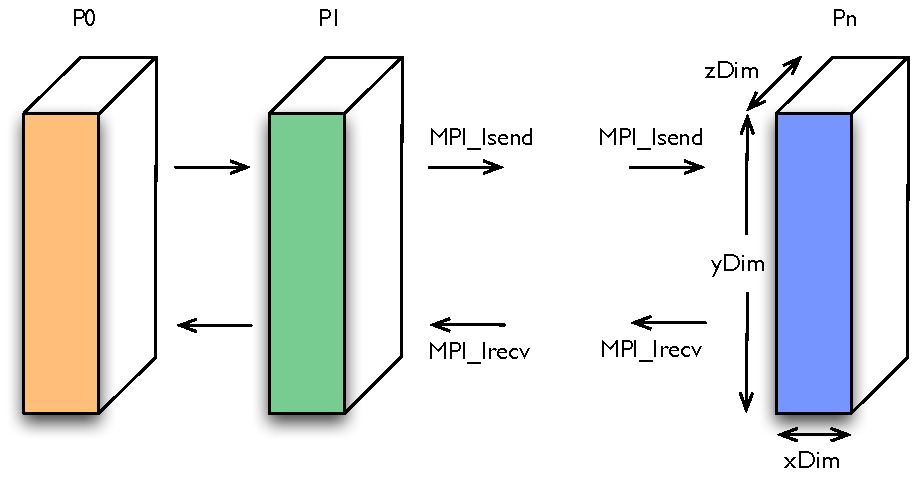
\includegraphics[width=\textwidth]{images/mpi_decomp}}
%\begin{center}
%Model bulk-synchronous Numerical Simulation
%\end{center}
%\end{frame}

%\begin{frame}
%\frametitle{Model Bulk-Synchronous MPI+OpenMP Application Code}
%\begin{center}
%\begin{figure}[ht]
%\lstinputlisting{/Users/kale2/hybridscheduling/listings/omp-static.c}
%\end{figure}
%\end{center}
%\end{frame}



\comments{
\begin{frame}
\frametitle{Model Bulk-synchronous code }
\lstinputlisting{/Users/kale2/hybridscheduling/listings/mpi-bulk-synch.c}
\begin{center}
\includegraphics[scale=0.65]{/Users/kale2/hybridscheduling/images/appTimestep}
\end{center}
\end{frame}

\begin{frame}
\frametitle{Model Bulk-synchronous Hybrid MPI+OpenMP code }
\lstinputlisting{/Users/kale2/hybridscheduling/listings/omp-static.c}
\begin{center}
\includegraphics[scale=0.45]{/Users/kale2/hybridscheduling/images/emptySchedImage}
\end{center}
\end{frame}

\begin{frame}
\frametitle{Model Hybrid MPI+OpenMP Code}
\visible<1->{\lstinputlisting{/Users/kale2/hybridscheduling/listings/omp-static.c}}
\visible<2->{\includegraphics[scale=0.35]{/Users/kale2/hybridscheduling/images/legend-appTimestep}}
\end{frame}

\begin{frame}
\frametitle{Conceptual Diagram of Timestep }
%\lstinputlisting{/Users/kale2/hybridscheduling/listings/omp-static.c}
\includegraphics[scale=0.35]{/Users/kale2/hybridscheduling/images/legend-appTimestep}
\begin{center}
\includegraphics[scale=0.45]{/Users/kale2/hybridscheduling/images/appTimestep}
\end{center}
%\includegraphics[scale=0.35]{/Users/kale2/hybridscheduling/images/legend-twocol}
%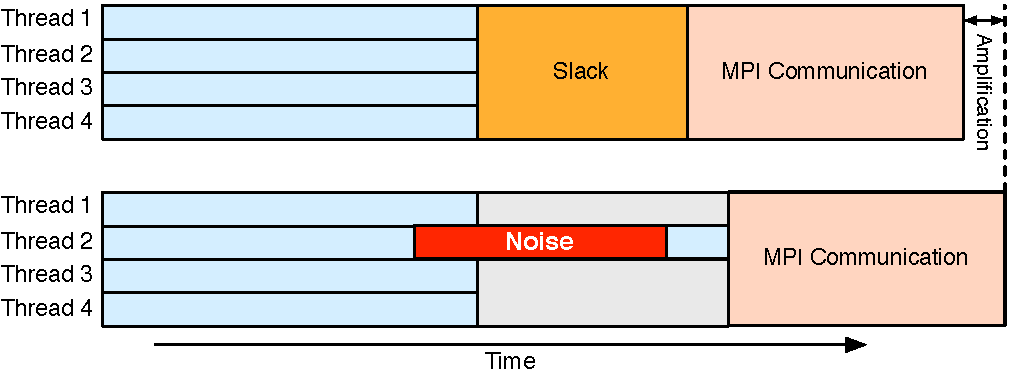
\includegraphics[scale=0.45]{/Users/kale2/hybridscheduling/images/static-schedule}
\begin{center}
\includegraphics[scale=0.45]{/Users/kale2/hybridscheduling/images/emptySchedImage}
\end{center}
\end{frame}

\begin{frame}
\frametitle{Amplification}
\includegraphics[scale=0.35]{/Users/kale2/hybridscheduling/images/legend-static}
\begin{center}
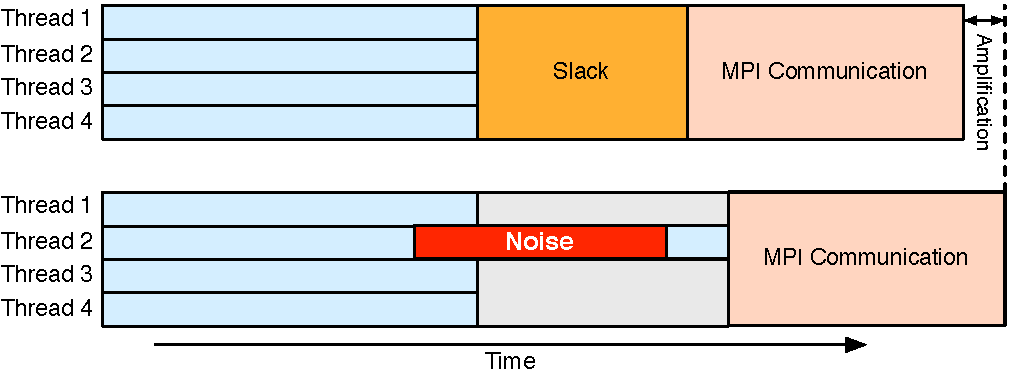
\includegraphics[scale=0.45]{/Users/kale2/hybridscheduling/images/static-schedule}
\end{center}
\begin{center}
\includegraphics[scale=0.45]{/Users/kale2/hybridscheduling/images/emptySchedImage}
\end{center}
\end{frame}


\begin{frame}
\frametitle{Assumption: Application is load balanced }
\begin{itemize}
\item \small Assume that problem is load balanced across MPI processes.
\item \small If problem isn't load balanced across MPI processes, then some other ``classical'' load balancer takes care of it.
\end{itemize}
\end{frame}

%\begin{frame}
%\frametitle{Localized Coordinated+Uncoordinated Load Imbalance}
%\begin{itemize}
%\item \small Assume that problem is load balanced across MPI processes.
%\item \small If problem isn't load balanced across MPI processes, then some other ``classical'' load balancer takes care of it.
%\item \small Imbalance stays within-node, or within racks
%\end{itemize}
%\end{frame}


\begin{frame}
\frametitle{Uncoordinated Transient Load Imbalance}
\begin{itemize}
\item \small If in iteration 304, if node 7 experiences excess work, it is not necessary that other nodes experience excess work in the same iteration.
\item \small If core 3 of node 7 has excess work, it does not mean core 3 of node 19 has excess work.
\item \small No pattern of load imbalances across MPI processes(show across space).
\end{itemize}
\end{frame}

\begin{frame}
\frametitle{Traditional load balancers are of no help }
\begin{enumerate}
\item \small Traditional load balancers,e.g. Measurement-based load balancer, handle load imbalances that persist over time
\item \small Here, no patterns of load imbalance across time, so can't use measurement-based load balancing.
\item \small Load imbalance happens with a certain probability on a node.
\item \small On each timestep, load imbalance happens with higher probability as we scale (as probabilities add up).
\item \small The probability of load imbalance occurring in one timestep increases as we scale (as probabilities add up).
\end{enumerate}
\end{frame}

\begin{frame}
\frametitle{Localized Uncoordinated Transient Load Imbalance}
\begin{itemize}

\end{itemize}
\end{frame}

}


%1. TO DO: do excel simulation for noise amplification curves for delta, p and T.  Also, consider modified delta after mitigation .

%%2. TO DO :  do experimentation for check asynchronous collectives

%\begin{frame}
%\frametitle{Why not asynchronous collectives?}
%\begin{itemize}
%\item suppose you have fraction f of work(from the next timestep/iteration) that you can do before results of the collective are available . What is the impact on amplification?
%\item
%\end{itemize}
%\end{frame}

\comments{

\begin{frame}
\frametitle{ What is the right amount of dynamic scheduling to use?(theory) }
\begin{itemize}
\item theoretical analysis
\end{itemize}
\end{frame}


% add in where ROSE comes in, and source to source comes in.
% put in MPI application specifics and code
% put in impact of compiler (icc vs. gcc)

\begin{frame}
\frametitle{Resilient Scheduling Strategy Applied to Model Synchronous MPI+OpenMP Code}
\lstinputlisting{/Users/kale2/hybridscheduling/listings/omp-static.c}
\lstinputlisting{/Users/kale2/hybridscheduling/listings/omp-hybrid.c}
\end{frame}

\begin{frame}
\frametitle{High-level Software Design}
\includegraphics[width=\textwidth]{/Users/kale2/hybridScheduling/images/architecture}
\end{frame}

\begin{frame}
\frametitle{Scaling with Resilient Scheduling}
\begin{figure}[h]
\label{fig:app-scaling-hera}
\begin{center}
\includegraphics[width=\columnwidth]{/Users/kale2/hybridscheduling/plots/app-scaling-hera}
\end{center}
\begin{center}
\tiny Percent speedup of callsite strategy over baseline stat. sched. on sierra.
\end{center}
\end{figure}

\begin{figure}[h]
\label{fig:app-scaling-rzuseq}
\begin{center}
%\includegraphics[width=\columnwidth]{/Users/kale2/hybridscheduling/plots/app-scaling-rzuseq}
\includegraphics[width=\columnwidth]{plots/app-scaling-rzuseq}
\end{center}
\begin{center}
\tiny Percent speedup of callsite strategy over baseline stat. sched. on rzuseq.
\end{center}
\end{figure}

%\begin{itemize}
%\small \item \tiny \textit{Static-Hybrid} gives moderate perf gains, as can be seen in figure~\ref{fig:app-scaling-hera}.
%\item \tiny Resilient-Callpath gives best perf. gain of all slack-conscious strategies, as seen in figure~\ref{fig:app-scaling-hera}.
%\item \tiny Resilient-Coll and Resilient-Naive give limited perf gains, likely due to
%  mispredictions, which outweigh the overhead of the prediction.
%\item \tiny As seen in figure ~\ref{fig:app-scaling-rzuseq}, the \textit{Resilient-Callpath} method does not cause large degradations, showing
%that using the methodology does not interfere greatly with the performance of the application.
%\end{itemize}
\end{frame}
}


\end{document}
